\documentclass[xcolor=table,fleqn]{beamer}

\usetheme[secheader,compress]{Madrid} %Primary theme
\setbeamertemplate{headline}{}  % uncomment this line if do not want headline shown in every frame.

\usepackage{xcolor}
\usepackage{epsfig}
\usepackage{stackengine}
\usepackage{hyperref}
\usepackage{multirow}
\usepackage{graphicx}
\usepackage{amsfonts}
\usepackage{array}
\usepackage{ulem}
\usepackage{amsthm}
\usepackage{textpos}
\usepackage{subfigure}
\usepackage{graphicx}
\usepackage{pbox}
\usepackage{tikz}
\usetikzlibrary{shapes}
\usepackage{tabularx}
\usepackage{framed}
\usetikzlibrary{arrows}
\usepackage{amsmath}

\tikzset{
  main node/.style={circle,draw,font=\small},
  rectangle/.style={font=\small},
	empty/.style={edge from parent/.style={}}
}

\setlength{\mathindent}{0pt}

\makeatletter
\newcommand{\removelatexerror}{\let\@latex@error\@gobble}
\makeatother

\makeatletter
\def\dual#1{\expandafter\dual@aux#1\@nil}
\def\dual@aux#1/#2\@nil{\begin{tabular}[b]{@{}c@{}}#1\\#2\end{tabular}}
\makeatother

\let\proof\relax
\let\endproof\relax

%\setbeamertemplate{bibliography entry title}{}
%\setbeamertemplate{bibliography entry location}{}
%\setbeamertemplate{bibliography entry note}{}
%\setbeamertemplate{bibliography item}[text]

%%% Customize the footline of the title page
\makeatletter
\setbeamertemplate{footline}
{
  \leavevmode%
  \hbox{%
  \begin{beamercolorbox}[wd=.333333\paperwidth,ht=2.25ex,dp=1ex,center]{author in head/foot}%
    \usebeamerfont{author in head/foot}\insertshortauthor
									 %\beamer@ifempty{\insertshortinstitute}{}{(\insertshortinstitute)}
  \end{beamercolorbox}%
  \begin{beamercolorbox}[wd=.333333\paperwidth,ht=2.25ex,dp=1ex,center]{title in head/foot}%
    \usebeamerfont{title in head/foot}\insertshorttitle
  \end{beamercolorbox}%
  \begin{beamercolorbox}[wd=.333333\paperwidth,ht=2.25ex,dp=1ex,right]{date in head/foot}%
    \usebeamerfont{date in head/foot}\insertshortdate{}\hspace*{2em}
    \insertframenumber{} / \inserttotalframenumber\hspace*{2ex} 
  \end{beamercolorbox}}%
  \vskip0pt%
}
\makeatother

%%% Customize the title line of all pages except the title page
\addtobeamertemplate{frametitle}{}{%
\begin{textblock*}{100mm}(.85\textwidth,-1cm)

\includegraphics[height=1cm,width=2.3cm]{figs/UK_logo.png}
\end{textblock*}}


%%%%%%%%%%% BEGIN MACROS %%%%%%%%%%%%%%%%%%
\newcommand{\ifLparse}{\operatorname{:-}}
\newcommand{\cI}{\mathcal{I}}
\newcommand{\CD}{\mathit{CD}}
\newcommand{\SD}{\mathit{SD}}
\newcommand{\TD}{\mathit{TD}}
\newcommand{\cX}{\mathcal{X}}
\newcommand{\cL}{\mathcal{L}}
\newcommand{\cV}{\mathcal{V}}
\newcommand{\ninst}{\mathit{NonInst}}
\newcommand{\inst}{\mathit{Inst}}
\newcommand{\WS}{\mathit{WS}}
\newcommand{\iss}{\mathit{Iss}}
\newcommand{\un}{\mathit{un}}
\newcommand{\rk}{\mathit{rk}}
\newcommand{\cP}{\mathcal{P}}
\newcommand{\iTran}{\textit{Transportation}}
\newcommand{\iDest}{\textit{Destination}}
\newcommand{\deltap}[1]{\mathit{\Delta^P_#1}}
\newcommand{\sigmap}[1]{\mathit{\Sigma^P_#1}}
\newcommand{\vph}{\mathit{\varphi}}
\newcommand{\fn}[1]{\footnote{\tiny{#1}}}
\newcommand{\figref}[1]{Figure~\ref{fig:#1}}
\newcommand{\tit}[1]{\textit{#1}}
\newcommand{\tbf}[1]{\textbf{#1}}

\newcommand\subsetsim{\mathrel{%
  \ooalign{\raise0.2ex\hbox{$\subset$}\cr\hidewidth\raise-0.8ex\hbox{\scalebox{0.9}{$\sim$}}\hidewidth\cr}}}

\newcommand{\Fontalg}{\fontsize{7}{7.2}\selectfont}

\newcommand{\frameT}[2]{\frame{\frametitle{#1} #2}}
\newcommand{\frameTop}[2]{\frame[t]{\frametitle{#1} #2}}

\newcommand{\tab}{\hspace{1cm}}
\newcommand{\spaceor}{\hspace{5pt} \textbf{or} \hspace{5pt}}
\newcommand{\sidefigure}{.49\linewidth}

\makeatletter
\newenvironment<>{proofs}[1][\proofname]{%
    \par
    \def\insertproofname{#1\@addpunct{.}}%
    \usebeamertemplate{proof begin}#2}
  {\usebeamertemplate{proof end}}
\makeatother

\newcommand{\backupbegin}{
   \newcounter{framenumberappendix}
   \setcounter{framenumberappendix}{\value{framenumber}}
}
\newcommand{\backupend}{
   \addtocounter{framenumberappendix}{-\value{framenumber}}
   \addtocounter{framenumber}{\value{framenumberappendix}} 
}

\newtheorem{thm}{Theorem}

%%%%%%%%%%% END MACROS %%%%%%%%%%%%%%%%%%



\begin{document}

\title[Preference Trees]
	{Reasoning with Preference Trees over Combinatorial Domains}
\author[Liu and Truszczynski]{\linebreak \linebreak Xudong Liu and Miroslaw Truszczynski}
\institute{Department of Computer Science \\ University of Kentucky\\ Lexington, KY, USA}
\date[\today]{}

%%%%%%%%%%% BEGIN TITLE PAGE %%%%%%%%%%%%%%%%%%
\frame
{
	\titlepage
}
%%%%%%%%%%%% END TITLE PAGE %%%%%%%%%%%%%%%%%%

\section{Introduction}

\frameT{Contributions}{
	\begin{enumerate}
		\item We provide an alternative definition of \tit{preference trees}\fn{
						Fraser. \tit{Ordinal preference representations}, 1994.
						}, or \tit{P-trees},
					and formally introduce their \tit{compact} representations.
		\item We relate P-trees to existing preference formalisms such as
					\tit{lexicographic preference trees} (\tit{LP-trees}), 
					\tit{answer set optimization} (\tit{ASO}) and \tit{possibilistic 
					logic} (\tit{Poss-theories}).
		\item We study decision problems in the setting of P-trees and obtain computational
					complexity results.
	\end{enumerate}
}


\section{Preference Trees}

\subsection{Definition}
\frameT{Preference Trees}{
	\begin{itemize}
		\item Let $\cI$ be a set of binary issues. The \tbf{combinatorial domain}
					$\CD(\cI)$ is the set of \tit{outcomes} represented by
					complete and consistent sets of literals over $\cI$.
		\item A \tbf{P-tree} $T$ over $\CD(\cI)$
					is a binary tree whose nodes, other than the leaves, are labeled with
					propositional formulas over $\cI$.
%		\item Given an outcome $M \in \CD(\cI)$, the \tbf{leaf} $l_T(M)$
%					is the leaf reached by traversing the tree $T$ according to $M$.
%					When at a node $N$ labeled with $\varphi$, if $M\models \varphi$,
%					we descend to the left child of $N$; otherwise, to the right.
%		\item For $M, M'\in \CD(\cI)$, we have $M\succ_T M'$ if $l_T(M) \succ_T l_T(M')$,
%					and $M \approx_T M'$ if $l_T(M)=l_T(M')$. Outcome $M$ is \tbf{optimal} if 
%					there exists no $M'$ such that $M' \succ_T M$.
	\end{itemize}
}

\frameT{Example: Preferences over Vacations}{
	\begin{center}
		\tit{activity}: \{water-sports ($x_1$), hiking ($\neg x_1$)\},\\
		\tit{destination}: \{Florida ($x_2$), Colorado ($\neg x_2$)\},\\
		\tit{time}: \{summer ($x_3$), winter ($\neg x_3$)\},\\
		\tit{transportation}: \{car ($x_4$), plane ($\neg x_4$)\}.
	\end{center}

\vspace{-0.2cm}

	\begin{figure}[!ht]
	  \centering
      \begin{tikzpicture}[->,>=stealth',
	      level 1/.style={sibling distance=1.7cm, level distance=33pt},
	      level 2/.style={sibling distance=1cm, level distance=27pt}
	    ]
        \node [main node,inner sep=0pt] (1){$x_1 \!\! \equiv \!\! x_2$}
          child {node [main node,inner sep=5pt] (2) {$x_4$}
            child {node [rectangle,draw] (3) {}}
            child {node [rectangle,draw] (4) {}}
                            }
          child {node [main node,inner sep=5pt] (5) {$x_4$}
            child {node [rectangle,draw] (6) {}
                                    }
            child {node [rectangle,draw] (7) {}
                                    }
          };
      \end{tikzpicture}
	  \caption{A P-tree over vacations}
	\end{figure}
}

\frameT{Example: Preferences over Vacations}{
	\begin{center}
		\tit{activity}: \{water-sports ($x_1$), hiking ($\neg x_1$)\},\\
		\tit{destination}: \{Florida ($x_2$), Colorado ($\neg x_2$)\},\\
		\tit{time}: \{summer ($x_3$), winter ($\neg x_3$)\},\\
		\tit{transportation}: \{car ($x_4$), plane ($\neg x_4$)\}.
	\end{center}

\vspace{-0.2cm}

	\begin{figure}[!ht]
	  \centering
      \begin{tikzpicture}[->,>=stealth',
	      level 1/.style={sibling distance=1.7cm, level distance=33pt},
	      level 2/.style={sibling distance=1cm, level distance=27pt}
	    ]
        \node [main node,inner sep=0pt] (1){$x_1 \!\! \equiv \!\! x_2$}
          child [red] {node [main node,inner sep=5pt,black] (2) {$x_4$}
            child [black] {node [rectangle,draw] (3) {}}
            child {node [rectangle,draw,fill] (4) {}}
                            }
          child [green] {node [main node,inner sep=5pt,black] (5) {$x_4$}
            child {node [rectangle,draw,fill] (6) {}
                                    }
            child [black] {node [rectangle,draw] (7) {}
                                    }
          };
      \end{tikzpicture}
	  \caption{A P-tree over vacations}
	\end{figure}

\vspace{-0.5cm}

	Preferences:
	\vspace{-0.4cm}
	\begin{center}
		$\textcolor{red}{\neg x_1 \neg x_2x_3\neg x_4} \succ \textcolor{green}{x_1 \neg x_2x_3x_4}$
	\end{center}
}

\frameT{Compact Representation of P-trees}{
\begin{figure}[!ht]
	\centering
		\subfigure[Full]{
		\centering
		  \begin{tikzpicture}[->,>=stealth',
  	     level 1/.style={sibling distance=4.3cm, level distance=28pt},
  	     level 2/.style={sibling distance=2.2cm, level distance=28pt},
  	     level 3/.style={sibling distance=1.0cm, level distance=28pt},
  	     level 4/.style={sibling distance=0.5cm, level distance=28pt}]
		    \node [main node,inner sep=1.7pt] (1){$\varphi_1$}
		    child {node [main node,inner sep=1.7pt] (2) {$\varphi_2$}
		      child {node [main node,inner sep=1.7pt] (3) {$\varphi_3$}
		        child {node [main node,inner sep=1.7pt] (4) {$\varphi_4$}
  	          child {node [rectangle,draw] (16) {}}
  	          child {node [rectangle,draw] (17) {}}
						}
		        child {node [main node,inner sep=1.7pt] (5) {$\varphi_4$}
  	          child {node [rectangle,draw] (18) {}}
  	          child {node [rectangle,draw] (19) {}}
						}
					}
		      child {node [main node,inner sep=1.7pt] (6) {$\varphi_3$}
		        child {node [main node,inner sep=1.7pt] (7) {$\varphi_4$}
  	          child {node [rectangle,draw] (20) {}}
  	          child {node [rectangle,draw] (21) {}}
						}
		        child {node [main node,inner sep=1.7pt] (8) {$\varphi_4$}
  	          child {node [rectangle,draw] (22) {}}
  	          child {node [rectangle,draw] (23) {}}
						}
		      }
				}
		    child {node [main node,inner sep=1.7pt] (9) {$\varphi_2$}
		      child {node [main node,inner sep=1.7pt] (10) {$\varphi_3$}
		        child {node [main node,inner sep=1.7pt] (11) {$\varphi_4$}
  	          child {node [rectangle,draw] (24) {}}
  	          child {node [rectangle,draw] (25) {}}
						}
		        child {node [main node,inner sep=1.7pt] (12) {$\varphi_4$}
  	          child {node [rectangle,draw] (26) {}}
  	          child {node [rectangle,draw] (27) {}}
						}
					}
		      child {node [main node,inner sep=1.7pt] (13) {$\varphi_3$}
		        child {node [main node,inner sep=1.7pt] (14) {$\varphi_4$}
  	          child {node [rectangle,draw] (28) {}}
  	          child {node [rectangle,draw] (29) {}}
						}
		        child {node [main node,inner sep=1.7pt] (15) {$\varphi_4$}
  	          child {node [rectangle,draw] (30) {}}
  	          child {node [rectangle,draw] (31) {}}
						}
		      }
				}
				;
		  \end{tikzpicture}
		}%
		\subfigure[Compact]{
			\hspace{0.8cm}
			\begin{tikzpicture}[->,>=stealth',
  	     level 1/.style={sibling distance=4.3cm, level distance=28pt},
  	     level 2/.style={sibling distance=2.2cm, level distance=28pt},
  	     level 3/.style={sibling distance=1.0cm, level distance=28pt},
  	     level 4/.style={sibling distance=0.5cm, level distance=28pt}]
			  \node [main node,inner sep=1.7pt] (1){$\varphi_1$}
			    child {node [main node,inner sep=1.7pt] (3) {$\varphi_2$}
						child {node [main node,inner sep=1.7pt] (4) {$\varphi_3$}
							child {node [main node,inner sep=1.7pt] (5) {$\varphi_4$}
              	child {node [rectangle] (6) {} edge from parent[draw=none]}
							}
						}
					};
			\end{tikzpicture}
			\hspace{0.8cm}
		}
  \caption{Compact P-trees}
%	\vspace{-0.2cm}
  \label{fig:LPT_full}
\end{figure}
}

\frameT{Compact Representation of P-trees}{
	\begin{center}
		\tit{activity}: \{water-sports ($x_1$), hiking ($\neg x_1$)\},\\
		\tit{destination}: \{Florida ($x_2$), Colorado ($\neg x_2$)\},\\
		\tit{time}: \{summer ($x_3$), winter ($\neg x_3$)\},\\
		\tit{transportation}: \{car ($x_4$), plane ($\neg x_4$)\}.
	\end{center}

\vspace{-0.2cm}

	\begin{figure}
	  \centering
	  \subfigure[Full]{
	    \centering
      \begin{tikzpicture}[->,>=stealth',
	      level 1/.style={sibling distance=1.7cm, level distance=33pt},
	      level 2/.style={sibling distance=1cm, level distance=27pt}
	    ]
        \node [main node,inner sep=0pt] (1){$x_1 \!\! \equiv \!\! x_2$}
          child {node [main node,inner sep=5pt] (2) {$x_4$}
            child {node [rectangle,draw] (3) {}}
            child {node [rectangle,draw] (4) {}}
                            }
          child {node [main node,inner sep=5pt] (5) {$x_4$}
            child {node [rectangle,draw] (6) {}
                                    }
            child {node [rectangle,draw] (7) {}
                                    }
          };
      \end{tikzpicture}
	  }
	  \subfigure[Compact]{
			\hspace{0.5cm}
      \begin{tikzpicture}[->,>=stealth',
        level 1/.style={sibling distance=1.7cm, level distance=33pt},
        level 2/.style={sibling distance=1cm, level distance=27pt}]
        \node [main node,inner sep=0pt] (1){$x_1 \!\! \equiv \!\! x_2$}
          child {node [main node,inner sep=5pt] (2) {$x_4$}
                    child {node [rectangle] (4) {} edge from parent[draw=none]}
                            };
      \end{tikzpicture}
			\hspace{0.5cm}
	  }
	\caption{Compact P-trees}
	\end{figure}
}

\frameT{Compact Representation of P-trees}{
	\begin{center}
		$\vph_1=x_1 \lor x_3$, $\vph_2 =x_1 \land \neg x_2$, \\ $\vph_3= (x_3 \rightarrow x_4) \lor (\neg x_3 \rightarrow \neg x_4)$.
	\end{center}

	\vspace{-0.7cm}

	\begin{figure}
	  \centering
	  \subfigure[Full]{
	    \centering
	    \begin{tikzpicture}[->,>=stealth',
	      level 1/.style={sibling distance=2cm, level distance=27pt},
	      level 2/.style={sibling distance=1.5cm, level distance=27pt},
	      level 3/.style={sibling distance=1cm, level distance=27pt}
				]
	      \node [main node,inner sep=1.7pt] (1){$\varphi_1$}
	        child {node [main node,inner sep=1.7pt] (2) {$\varphi_2$}
	          child {node [main node,inner sep=1.7pt] (3) {$\varphi_3$}
	            child {node [rectangle,draw] (4) {}}
	            child {node [rectangle,draw] (5) {}}
           }
           child {node [main node,inner sep=1.7pt] (6) {$\varphi_3$}
	            child {node [rectangle,draw] (7) {}}
	            child {node [rectangle,draw] (8) {}}
	          }
	        }
%	        child [empty] {}
	        child {node [rectangle,draw] (9) {}}
	        ;
	    \end{tikzpicture}
	  }
	  \subfigure[Compact]{
			\hspace{0.4cm}
	    \begin{tikzpicture}[->,>=stealth',
	      level/.style={sibling distance=2cm, level distance=27pt}]
	      \node [main node,inner sep=1.7pt] (1){$\varphi_1$}
	        child {node [main node,inner sep=1.7pt] (2) {$\varphi_2$}
	          child {node [main node,inner sep=1.7pt] (3) {$\varphi_3$}
	        		child [empty] {}
	          }
	        }
	        child [empty] {
	        };
	    \end{tikzpicture}
	  }
	\caption{Compact P-trees}
	\end{figure}
}

\frameT{Compact Representation of P-trees}{
	A \tit{compact P-tree over $\CD(\cI)$} is a tree where
	\begin{enumerate}
		\setlength\itemsep{0em}
		\item every node is labeled with a Boolean formula over $\cI$, and
	  \item every non-leaf node $t$ labeled with $\varphi$ has either
	        two outgoing edges (Figure (a)), or one 
	    		outgoing edge pointing left (Figure (b)),
					right (Figure (c)), or straight-down (Figure (d)).
	\end{enumerate}
	
	\begin{figure}[ht!]
	  \centering
	    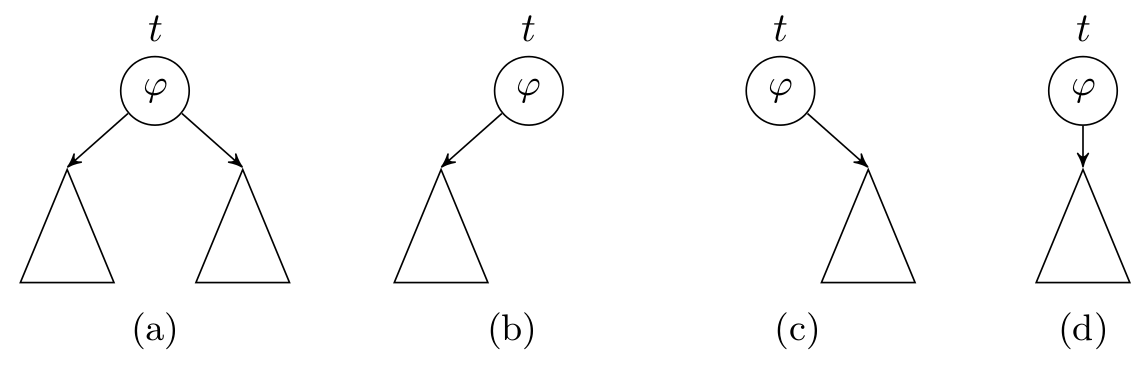
\includegraphics[width=0.9\textwidth]{figs/ptrees.png}
	  \caption{Compact P-trees}
	\end{figure}
}


\subsection{Relating Other Preference Formalisms}
\frameT{From LP-Trees\fn{
	Booth, Chevaleyre, Lang, Mengin, and Sombattheera.
	\tit{Learning conditionally lexicographic preference relations}, 2010.
} to P-Trees}{
	\begin{figure}[!ht]
		\centering
	  \subfigure[An LP-tree $L$]{
			\centering
		  \begin{tikzpicture}[->,>=stealth',node distance=1.4cm]
		        
		    \node[main node,inner sep=2pt] (1) {$X_1$};
		    \node[rectangle,draw,inner sep=2pt,font=\sffamily\tiny] at (-1,0) {$x_1 > \neg x_1$};
		
		    \node[main node,inner sep=2pt] (2) [below of=1] {$X_3$};
		    \node[rectangle,draw,inner sep=2pt,font=\sffamily\tiny] at (-1,-1.4) {$x_3 > \neg x_3$};
		    
		    \node[main node,inner sep=2pt] (3) [below left of=2] {$X_2$};
		    \node[rectangle,draw,inner sep=2pt,font=\sffamily\tiny] at (-1.9,-2.4) {$\neg x_2 > x_2$};
		    
		    \node[main node,inner sep=2pt] (4) [below of=3] {$X_4$};
		    \node[rectangle split, rectangle split parts=2, draw,font=\sffamily\tiny,inner sep=2pt] at (-2.3,-3.8)
		        {
		          $x_2:x_4 > \neg x_4$
		          \nodepart{second}
		          $\neg x_2:\neg x_4 > x_4$
		        };
		    
		    \node[main node,inner sep=2pt] (5) [below right of=2] {$X_4$};
		    \node[rectangle,draw,inner sep=2pt,font=\sffamily\tiny] at (0.05,-2.4) {$\neg x_4 > x_4$};
		    
		    \node[main node,inner sep=2pt] (6) [below of=5] {$X_2$};
		    \node[rectangle,draw,inner sep=2pt,font=\sffamily\tiny] at (0.05,-3.8) {$x_2 > \neg x_2$};
		  
		    \path[every node/.style={font=\sffamily\small}]
		      (1) edge (2)
		      (2) edge (3)
		          edge (5)
		      (3) edge (4)
		      (5) edge (6);
		  \end{tikzpicture}
		} \quad \quad
		\subfigure[The P-tree $T_L$\protect\footnotemark]{
				\hspace{0.5cm}
			  \begin{tikzpicture}[->,>=stealth',
			    level/.style={sibling distance=1.5cm, level distance=30pt}]
			    \node [main node] (1){$x_1$}
			    child {node [main node] (2) {$x_3$}
			      child {node [main node,inner sep=1.5pt] (3) {$\neg x_2$}
			        child {node [main node,inner sep=4pt] (4) {$\varphi$}
							}
						}
			      child {node [main node,inner sep=1.5pt] (6) {$\neg x_4$}
			        child {node [main node] (7) {$x_2$}
							}
			      }};
			  \end{tikzpicture}
				\hspace{0.5cm}
			}
	  \caption{P-trees embed LP-trees}
	\end{figure}
	\footnotetext{\tiny{$\varphi=(x_2 \rightarrow x_4) \vee (\neg x_2 
								\rightarrow \neg x_4)$}}
}

%\frameT{Answer Set Optimization (ASO)}{
%	\begin{itemize}
%		\item An ASO-rule
%					$r$ over $\cI$ is a preference rule of the form
%					\begin{center} \label{eq:ASO}
%						$C_1 > \ldots > C_m \leftarrow B$,
%					\end{center}
%					where all $C_i$'s and $B$ are propositional formulas over $\cI$.
%		\item For an outcome $M \in \CD(\cI)$, the rule determines its \tit{satisfaction 
%					degree}\fn{This definition is a slight adaptation of the original one.},
%					denoted by $\SD_r(M)$ such that
%					\begin{center}
%					$
%					\small{\SD_r(M) =
%					  \begin{cases}
%					   1, & M \models \neg B \\
%					   m+1, & M \models B \wedge \bigwedge_{1 \leq i \leq m} \neg C_i \\
%					   min\{i:M \models C_i\}, & \mbox{otherwise}.
%					  \end{cases}}
%					$
%					\end{center}
%		\item	$M \succeq_r M'$ if $\SD_r(M)\leq\SD_r(M')$. 
%					%Thus, the ASO-rule partitions outcomes into $m+1$ clusters.
%	\end{itemize}
%
%}

%\frameT{Example ASO-rule over Vacations}{
%	\begin{center}
%		\tit{activity}: \{water-sports ($x_1$), hiking ($\neg x_1$)\},\\
%		\tit{destination}: \{Florida ($x_2$), Colorado ($\neg x_2$)\},\\
%		\tit{time}: \{summer ($x_3$), winter ($\neg x_3$)\},\\
%		\tit{transportation}: \{car ($x_4$), plane ($\neg x_4$)\}.
%	\end{center}
%
%\vspace{-0.2cm}
%
%	\begin{center}
%		$r:\,\,x_1 \equiv x_2 > x_3 > x_2 \leftarrow$.
%	\end{center}
%
%	We have the following preferences:
%
%	\begin{center}
%		$\SD_r(x_1x_2x_3x_4)=\SD_r(\neg x_1\neg x_2x_3x_4)=1$:\\
%		$x_1x_2x_3x_4 \approx_r \neg x_1\neg x_2x_3x_4$.\\
%		$\SD_r(\neg x_1x_2\neg x_3\neg x_4)=3$, $\SD_r(x_1\neg x_2\neg x_3x_4)=4$:\\
%		$\neg x_1x_2\neg x_3\neg x_4 \succ_r x_1\neg x_2\neg x_3x_4$.
%	\end{center}
%}

\frameT{From ASO-Rules\fn{
	Brewka, Niemel¨a, and Truszczynski. \tit{Answer set optimization}, 2003.
} to P-Trees}{
	From the ASO-rule $r$, we build a P-tree $T_r$,
	where $\varphi_1 = \neg B \vee C_1$,
	$\varphi_i =C_i$ ($2 \leq i \leq m$).
	
	\vspace{-0.2cm}
	\begin{figure}
	  \small
	  \centering
	  \subfigure[ASO-rule $r$]{
			\raisebox{10mm}{
			$C_1 > \ldots > C_m \leftarrow B$
			}
	  }
		\subfigure[P-tree $T_r$]{
		  \begin{tikzpicture}[->,>=stealth',
		    level 1/.style={sibling distance=1.5cm, level distance=27pt},
		    level 2/.style={sibling distance=1.5cm, level distance=27pt}
				]
		    \node [main node,inner sep=1.7pt] (1){$\varphi_1$}
		      child [empty] {}
		      child {node [main node,inner sep=1.7pt] (3) {$\varphi_2$}
		      	child [empty] {}
						child {node [main node,inner sep=0.9pt] (5) {$\varphi_m$} [dashed]
						}
					};
		  \end{tikzpicture}
		}
	\caption{P-trees embed ASO-rules}
	\end{figure}
	\vspace{-0.5cm}

	\begin{thm}
		Given an ASO-rule $r$, there exists a P-tree $T_r$ of size
		polynomial in the size of $r$ such that for every two outcomes $o$ and $o'$
			\vspace{-0.2cm}
		\begin{center}
			$o \succeq_r o' \;\; \tit{iff} \;\; o \succeq_{T_r} o'$
		\end{center}
	\end{thm}
}

\frameT{From P-Trees to ASO-Rules?}{
	\begin{figure}
	  \small
	  \centering
		  \begin{tikzpicture}[->,>=stealth',
		    level 1/.style={sibling distance=1.5cm, level distance=32pt},
		    level 2/.style={sibling distance=1cm, level distance=32pt}
				]
		    \node [main node,inner sep=1.7pt] (1){$\varphi_1$}
		      child {node [main node,inner sep=1.7pt] (3) {$\varphi_2$}
						child {node [main node,inner sep=0.9pt] (5) {$\varphi_m$} [dashed]
						}
					};
		  \end{tikzpicture}
	  \caption{A P-tree $T$}
	\end{figure}

	\begin{center}
		$r_T: \underbrace{\varphi_1 \land \ldots \land \varphi_m >
		 \varphi_1 \land \ldots \land \neg \varphi_m >
		 \ldots > \neg \varphi_1 \land \ldots \land 
		 \neg \varphi_m}_{\text{\large TOO many formulas!}}$
	\end{center}
}

%\frameT{Ranked Answer Set Optimization (RASO)}{
%	\begin{itemize}
%		\item An (unranked) ASO-theory, or ASO-theory, $P$ is a set of ASO-rules
%					aggregated by the Pareto method.
%		\begin{enumerate}
%			\item $M \succeq_P^\un M'$ if $\SD_r(M) \leq \SD_r(M')$ for every
%						$r \in P$.
%			\item $M \succ_P^\un M'$ if $M \succeq_P^\un M'$ and $\SD_r(M) < \SD_r(M')$ for some
%						$r \in P$.
%			\item $M \approx_P^\un M'$ if $\SD_r(M) = \SD_r(M')$ for every
%						$r \in P$.
%		\end{enumerate}
%	\end{itemize}
%
%	\begin{itemize}
%		\item An ranked ASO-theory\fn{
%						Brewka, Niemel¨a, and
%						Truszczynski. \tit{Answer set optimization}, 2003.},
%					or RASO-theory, $P=\{P_1,\ldots,P_g\}$ is a set of ASO-rules
%					with $g$ ranks, the smaller the rank the more important the rules.
%		\begin{enumerate}
%			\item $M \succeq^\rk_P M'$ if for every $i$, $1\leq i\leq g$, 
%						$M \approx^\un_{P_i} M'$, or if there exists a rank $i$ such that 
%						$M \approx^\un_{P_j} M'$ for every $j$, $j< i$, and $M \succ^\un_{P_i} M'$.
%		\end{enumerate}
%	\end{itemize}
%
%}

%\frameT{Example ASO-theory over Vacations}{
%	\begin{center}
%		\tit{activity}: \{water-sports ($x_1$), hiking ($\neg x_1$)\},\\
%		\tit{destination}: \{Florida ($x_2$), Colorado ($\neg x_2$)\},\\
%		\tit{time}: \{summer ($x_3$), winter ($\neg x_3$)\},\\
%		\tit{transportation}: \{car ($x_4$), plane ($\neg x_4$)\}.
%	\end{center}
%
%\vspace{-0.2cm}
%
%\begin{equation*}
%\hspace{3.2cm}
%\Phi =
%\begin{cases}
%r_1:\,\,x_1 \equiv x_2 > x_3 \overset{1}{\leftarrow},
%\\
%r_2:\,\,x_4 \land x_2 > x_4 \land \neg x_2 \overset{2}{\leftarrow}.
%\end{cases}
%\end{equation*}
%
%	We have the following preferences:
%	\begin{center}
%		$\SD_\Phi(x_1x_2\neg x_3x_4)=[1,1]$, $\SD_\Phi(\neg x_1\neg x_2x_3\neg x_4)=[1,3]$:\\
%		$x_1x_2\neg x_3x_4 \succ_\Phi \neg x_1\neg x_2\neg x_3x_4$.
%	\end{center}
%}
%

\frameT{From P-trees to ASO-Theories\fn{
	Brewka, Niemel¨a, and Truszczynski. \tit{Answer set optimization}, 2003.
}}{
	\begin{figure}
	  \centering
	  \subfigure[P-tree $T$]{
			\hspace{0.5cm}
      \begin{tikzpicture}[->,>=stealth',
        level 1/.style={sibling distance=1.7cm, level distance=33pt},
        level 2/.style={sibling distance=1cm, level distance=27pt}]
        \node [main node,inner sep=0pt] (1){$x_1 \!\! \equiv \!\! x_2$}
          child {node [main node,inner sep=5pt] (2) {$x_4$}
                            };
      \end{tikzpicture}
			\hspace{0.5cm}
	  }
		\subfigure[ASO-theory $\Phi_T$]{
			\hspace{0.5cm}
			\begin{tikzpicture}[->,>=stealth,node distance=0.5cm,main node/.style={rectangle,font=\small}]
		    \node[main node] (1) {$x_1 \equiv x_2 \overset{1}{\leftarrow}$,};
		    \node[main node] (2) [below of=1] {$x_4 \overset{2}{\leftarrow}$.};
		  \end{tikzpicture}
			\hspace{0.5cm}
		}
	\caption{ASO-theories embed P-trees}
	\end{figure}

	\vspace{-0.5cm}

	\begin{thm}
		Given a P-tree $T$, there exists an ASO-theory $\Phi_T$ of size
		polynomial in the size of $T$ such that for every two outcomes $o$ and $o'$
		\begin{center}
			$o \succeq_{\Phi_T} o' \;\; \tit{iff} \;\; o \succeq_{T} o'$
		\end{center}
	\end{thm}
}

%\frameT{P-Trees and Possibilistic Logic}{
%	\begin{enumerate}
%		\item A possibilistic logic theory $\Pi$ over a vocabulary $\cI$ is a set of pairs
%					\begin{center}
%						$\{ (\phi_1,a_1), \ldots, (\phi_m,a_m) \}$,
%					\end{center}
%					where every $\phi_i$ is a Boolean formula over $\cI$, and every $a_i$,
%					the importance of $\phi_i$, is a real number
%					such that $1\geq a_1>\ldots>a_m\geq 0$.
%		\item The \tit{tolerance degree} $\TD_{(\phi,a)}(M)$ of outcome $M$ with regard
%					to preference pair $(\phi,a)$:
%					\begin{center}
%					$
%					 \TD_{(\phi,a)}(M) =
%					  \begin{cases}
%					   1, & M \models \phi \\
%					   1-a, & M \not \models \phi
%					  \end{cases}
%					$
%					\end{center}
%		\item The tolerance degree $\TD_\Pi(M)$ of outcome $M$ w.r.t the possibilistic logic theory $\Pi$: 
%					\begin{center}
%						$\TD_\Pi(M)=min\{\TD_{(\phi_i,a_i)}(M):1\leq i \leq m\}$.
%					\end{center}
%		\item $M \succeq_\Pi M'$ if $\TD_\Pi(M) \geq \TD_\Pi(M')$.
%	\end{enumerate}
%}

\frameT{From Poss-theories\fn{
						Dubois, Lang, and Prade.
						\tit{A brief overview of possibilistic logic}, 1991.
} to P-Trees}{
	Given a possibilistic logic theory $\Pi$, we now build a P-tree $T_\Pi$, 
	where $\varphi_1=\bigwedge_{\substack{1\leq i \leq m}} \phi_i$, 
	$\varphi_2=\bigwedge_{\substack{1\leq i \leq m-1}} \phi_i \wedge \neg \phi_m$,
	$\varphi_3=\bigwedge_{\substack{1\leq i \leq m-2}} \phi_i \wedge \neg \phi_{m-1}$, and
	$\varphi_m = \phi_1 \wedge \neg \phi_2$.

	\vspace{-0.3cm}
	\begin{figure}
	  \small
	  \centering
	  \subfigure[Poss-theory $\Pi$]{
			\raisebox{10mm}{
				$\{ (\phi_1,a_1), \ldots, (\phi_m,a_m) \}$
			}
	  }
		\subfigure[P-tree $T_\Pi$]{
		  \begin{tikzpicture}[->,>=stealth',
		    level 1/.style={sibling distance=1.5cm, level distance=27pt},
		    level 2/.style={sibling distance=1.5cm, level distance=27pt}
				]
		    \node [main node,inner sep=1.7pt] (1){$\varphi_1$}
		      child [empty] {}
		      child {node [main node,inner sep=1.7pt] (3) {$\varphi_2$}
		      	child [empty] {}
						child {node [main node,inner sep=0.9pt] (5) {$\varphi_m$} [dashed]
						}
					};
		  \end{tikzpicture}
		}
	\caption{P-trees embed Poss-theories}
	\end{figure}
	\vspace{-0.6cm}
	\begin{thm}
		Given a possibilistic theory $\Pi$, the P-tree $T_\Pi$ is built in time
		polynomial in the size of $\Pi$ such that for every two outcomes $o$ and $o'$
		\begin{center}
			$o \succeq_\Pi^{\tit{Poss}} o' \;\; \tit{iff} \;\; o \succeq_{T_\Pi} o'$
		\end{center}
	\end{thm}
}

\frameT{Relative Expressivity of Preference Languages}{
	\begin{center}
		Poss-theories = ASO-rules $\subset$ \dual{LP-trees/\dual{$\cap$/P-trees}} $\subset$ ASO-theories \\
		P-trees $\subseteq$ Pen-theories
	\end{center}
}


\section{Decision Problems and Complexity}

\frameT{Decision Problems}{
	\begin{block}{Dominance-testing ({\sc DomTest})}
		Given a P-tree $T$ and its two distinct outcomes
		$o$ and $o'$, decide whether $o' \succeq_T o$.
	\end{block}
	
	\vspace{0.05cm}
	
	\begin{block}{Optimality-testing ({\sc OptTest})}
		Given a P-tree $T$ and an outcome $o$,
		decide whether $o$ is an optimal outcome with respect to $T$.
	\end{block}
	
	\vspace{0.05cm}
	
	\begin{block}{Optimality-with-property ({\sc OptProp})}
		Given a P-tree $T$ and some property $\alpha$
		expressed as a Boolean formula,
		decide whether there is an optimal outcome that satisfies $\alpha$.
	\end{block}
}

\frameT{Computational Complexity Results}{
	{\sc DomTest}: is it that $o \succeq_T o'$ in P-tree $T$?\\
	{\sc OptTest}: is outcome $o$ optimal w.r.t $T$?\\
	{\sc OptProp}: is there an optimal outcome $o$ w.r.t $T$ st $o \models \alpha$?
	
	\begin{figure}
		\centering

	  \begin{tabular}[0.5\textwidth]{ | c | c | c | c | }
	    \hline
	     & {\sc DomTest}& {\sc OptTest} & {\sc OptProp} \\
			\hline
			LP-tree & P & P & P \\
			\hline
			\pbox{20cm}{ASO-rule/ \\ Poss-theory} & P & coNP-c & $\deltap{2}$($P^{NP}$) \\
	    \hline
	    \tbf{P-tree} & \tbf{P} & \tbf{coNP-c}\fn{The complement problem is reduced from the SAT problem.}
				& \tbf{$\deltap{2}$($P^{NP}$)-c}\fn{The problem is reduced from the Maximum Satisfying 
																					Assignment (MSA) problem.}\\
			\hline
			ASO-theory & P & coNP-c & $\sigmap{2}$($NP^{NP}$)-c \\
	    \hline
			%ACP-net & NP-hard & P & P \\
	    %\hline
			%CCP-net & PSPACE-c & PSPACE-c? & PSPACE-c? \\
	    %\hline
	  \end{tabular}

		\caption{Computational complexity results}

	\end{figure}
}


\section{Future Work}

\frameT{Future Work}{
\begin{enumerate}
	\item Relating P-trees with CP-nets\fn{
						Boutilier et al.
						\tit{CP-nets: A tool for representing
						and reasoning with conditional ceteris paribus
						preference statements}, 2004.
					}.
	\item Eliciting and learning P-trees.
	\item Aggregating P-trees: the Pareto method, social choice rules.
\end{enumerate}

\vspace{3cm}

\hspace{8cm} Questions? Thank you!
}



\end{document}
